\documentclass[12pt]{article}

\usepackage[a4paper, margin=1in]{geometry}
\usepackage{xcolor}
\usepackage{tcolorbox}
\usepackage{fontawesome5} % icons
\usepackage{hyperref}
\usepackage{graphicx}
\usepackage{comment}
\usepackage[nameinlink,capitalize,noabbrev]{cleveref}

\setlength{\parindent}{0pt}

% --- COLOR PALETTE (customize these) ---
\definecolor{maincolor}{HTML}{2A9D8F} % your teal
\definecolor{accentcolor}{HTML}{E76F51}
\definecolor{lightcolor}{HTML}{FFDEAD}

% Tell cleveref how to name your counter
\crefname{exercise}{assignment}{assignments}
\Crefname{exercise}{Assignment}{Assignments}

% --- ASSIGNMENT STYLE ---
\newcounter{exercise}

% Optional label: \exercisetitle[<label>]{<Title>}
\newcommand{\exercisetitle}[2][]{%
  \refstepcounter{exercise}% make this step referenceable/hyperlinked
  \vspace{0.5cm}%
  \colorbox{maincolor}{%
    \makebox[\dimexpr\linewidth-2\fboxsep][l]{%
      \textcolor{white}{\faPen\ Assignment \theexercise:~ #2}%
    }%
  }%
  % If an optional label was provided, set it
  \if\relax\detokenize{#1}\relax\else\label{#1}\fi
  \vspace{0.3cm}%
}

% --- IMPORTANT BOX ---
\newtcolorbox{importantbox}{
  colback=lightcolor,
  colframe=accentcolor,
  arc=4mm,
  boxrule=1pt,
  left=6pt,
  right=6pt,
  top=6pt,
  bottom=6pt
}

% --- PROMPT BOX ---
\newtcolorbox{promptbox}{
  colback=white,
  colframe=maincolor,
  arc=4mm,
  boxrule=1pt,
  left=6pt,
  right=6pt,
  top=6pt,
  bottom=6pt
}

% --- QUESTION BOX ---
\newcounter{question}

\newcommand{\question}[2][5cm]{%
  \stepcounter{question}
  \vspace{0.3cm}
  \textbf{\faEdit\ Question \thequestion: #2} \\[0.3em]
  
  \begin{Form}
  \TextField[
    name=Q\thequestion,
    multiline=true,
    width=\linewidth,
    height=#1,
    charsize=10pt,
    bordercolor={0 0 0},
    borderwidth=1.8,
    backgroundcolor={1 1 1}
  ]{}
  \end{Form}
  
  \vspace{0.3cm}
}

% --- SOLUTION BOX ---
%--- Definition of solution/no solution env to change between the teacher and the student versions --------%

% --- Teacher toggle ---
\newif\ifteacher
\teachertrue  % Write teacherfalse for student version and teachertrue for teachers version

% --- Solution environment ---
\newtcolorbox{solutionbox}{colback=gray!10,colframe=black!60!black,arc=1mm,boxrule=1pt}

\ifteacher
\newenvironment{solution}{%
  \begin{solutionbox}\textbf{Solution:}
}{%
  \end{solutionbox}
}
\else
  \excludecomment{solution}
\fi


\begin{document}

\begin{titlepage}

% --- Top spacing ---
\vspace*{1cm}

% --- Project logo ---
\begin{center}
    
\includegraphics[height=3cm]{Figures/Logo_TAI_Transparent.png}
\end{center}

\vspace{0.8cm}

% --- Title page ---
\begin{center}
    {\Huge \bfseries \color{maincolor} Diffusion models\par}
    \vspace{0.5cm}
    
    {\Large \color{accentcolor} Teaching with AI (TAI) \par}
    
    \vspace{1.5cm}
    
    \begin{center}
{\large
Mirte van der Eyden$^{1}$, Andrea López Incera$^{2}$ \\[0.3cm]

{\small
$^{1}$ Institut für Fachdidaktik, Universität Innsbruck \\ 
mirte.van-der-eyden@uibk.ac.at \\[0.2cm]


$^{2}$ Departament de didàctica de la matemàtica i les ciències experimentals, Universitat Autònoma de Barcelona \\ 
andrea.lopez.incera@uab.cat
}
}
\end{center}

\end{center}

\vfill

% --- Logos at the bottom ---
\begin{center}
\begin{tabular}{ccc}

\includegraphics[height=1.5cm]{Figures/Logos/universitaet-innsbruck-logo-cmyk-farbe.jpg} &

\includegraphics[height=1.5cm]{Figures/Logos/logotipuab-v1-verd.png} &

\includegraphics[height=1.5cm]{Figures/Logos/EN Co-funded by the EU_POS.jpg}
\end{tabular}
\end{center}


\vspace{0.5cm}

% Optional footer text
\begin{center}
    {\small Project funded by Erasmus+ Programme of the European Union}
\end{center}

\end{titlepage}

% --- Description of activity ---
\vspace*{0.5\textheight}

Subject: The basic principles of diffusion models

Activity duration: 45 min

\vspace{0.5cm}

Steps:
\begin{enumerate}
\item Initial discussion (5 min)
  \item Recovering an image that was hidden in noise (15 min)
  \item Diffusion: How it works (15 min)
  \item Visualization of the diffusion process (10 min)
\end{enumerate}

Learning goals:

\begin{itemize}
  \item Understanding how AI models generate images with the diffusion mechanism
\end{itemize}

Setup:
\begin{itemize}
  \item Per 2/3 students: a computer with access to an AI image generation tool. 
  \item Printed sheets and stickers for \Cref{ass:offline}.
\end{itemize}
\newpage

% --- HEADER / BRANDING ---
\begin{center}
    {\Huge \color{maincolor} Diffusion models}\\[5pt]
    {\large \textit{The basic principles}}\\
    \rule{\linewidth}{1pt}
\end{center}

\vspace{0.5cm}

How do AI models generate images, music and videos? Behind it is a diffusion model that can generate structure out of noise. In this lesson you learn how it works.

\exercisetitle{Initial discusssion}

Discuss the following questions in small groups or in class: 
\begin{itemize}
    \item What is your experience with generating images with AI?
    \item Can you describe an image you made that you liked?
    \item Do you have an example of an image that came out wrong or weird?
\end{itemize}



% --- Assignment ---
\exercisetitle{An imgage hidden in the noise}\label{ass:offline}

\begin{figure}[h]
    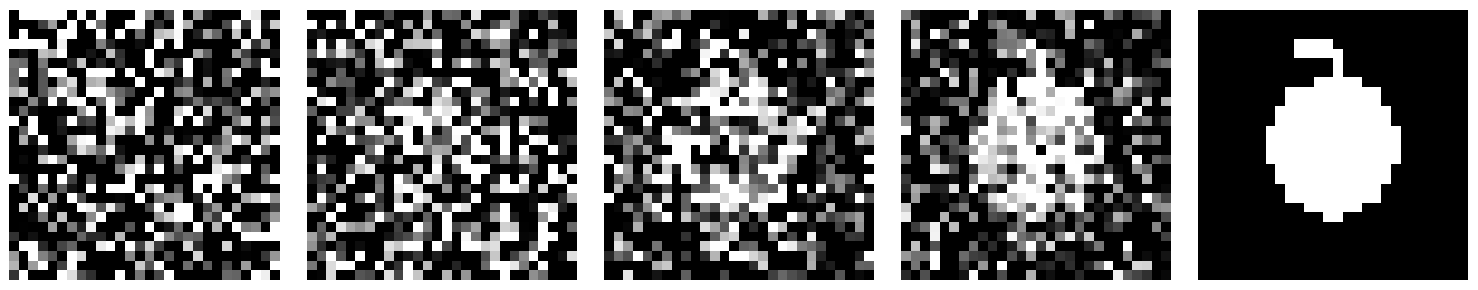
\includegraphics[width=\textwidth]{Figures/diffusion/apple_from_noise.png}
    \caption{A picture of an apple appears from the noise.}
    \label{fig:apple_from_noise}
\end{figure}



Form groups of 5 or 6 students. Everyone receives a sheet printed with a noisy figure and a prompt written on top, as well as sheets of black and white stickers. 

Somewhere in the noise, there is an image of hidden that depicts the prompt. The sheet you obtain is created like \cref{fig:apple_from_noise}, and is in stage 3, like the middle image of the noisy apple. 

Try to create that image of the prompt, by changing pixels. Every step of 30 seconds, you do the following:
\begin{enumerate}
  \item Read the prompt on top. 
  \item Make some changes to the pixels by pasting black or white stickers, such that the image starts looking more like the prompt. 
  \item If you do not know where to start, it sometimes helps to look through your eyelids for an already existing shape. 
  \item Do not draw lines, only fill/erase pixels with stickers. 
  \item At the end of the 30 seconds, give the sheet to your neighbour on the left.
\end{enumerate}

After 10 rounds we collect all drawings in front of the classroom. Discuss the following questions:
\begin{itemize}
  \item Do you recognize the images?
  \item How did you decide where to make changes?
  \item What differences and similarities do you notice between the examples of the same prompts?
  \item You will obtain the actual starting image that was used to create your noisy sheet. Compare the differences. 
  \item How do you imagine that a computer can create an image out of noise?
\end{itemize}


\section{Generating images}

You might have some experience in generating images with AI. Nowadays, this is extremely easy. You just tell the AI what you want to have, for example:  

\vspace{0.3cm}
\textcolor{maincolor}{\textbf{\faCopy\ Prompt}}
\begin{promptbox}Picture of a cute cat riding a bicycle.
\end{promptbox}

This prompt resulted in \cref{fig:cat} using the AI image generation tool of Canva. 

\begin{figure}[h]
    \centering
    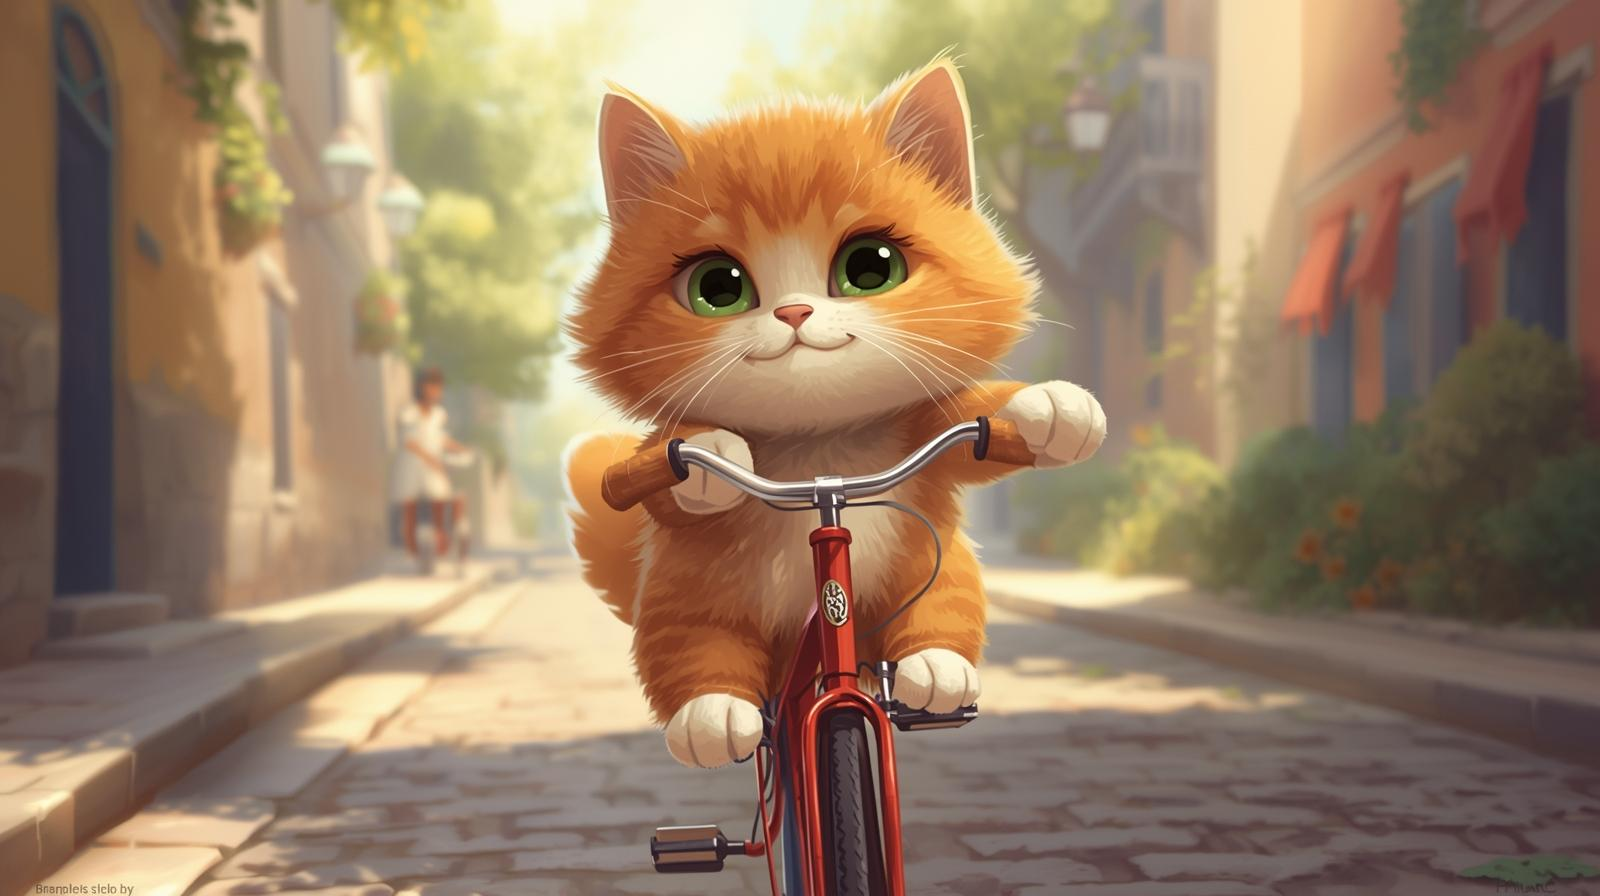
\includegraphics[width=0.5\linewidth]{Figures/diffusion/cat_on_bike.jpg}
    \caption{An AI generated image of a `cute cat riding a bicycle'.}
    \label{fig:cat}
\end{figure}

\exercisetitle{Generating images}

Go to an AI platform that generates images (ChatGPT, Canva, .. ) and generate an image of your favorite animal playing your favorite sport. 

\question[3cm]{Prompt:}

The generation of the image you just created, consists of different steps. Those steps are covered in different lessons:

\begin{enumerate}
    \item How does the AI understand my textual input? (Topic of lesson "How LLMs work")
    \item Once it understands what I want to create, how does the AI create an image from scratch? (Topic of this lesson)
    \item How can I best write a prompt such that I get the image I want? (Topic of lesson "How to prompt: images")
\end{enumerate}

In this lesson, we focus on the second question: how are images created with AI? Most of the image generation tools work in the same way: they use Diffusion models.

\section{Diffusion models explained}



\subsection{From pixel to picture}

We as humans can observe images, their colors, shapes and sizes, in a way that seems continuous. In a computer, an image is built up from pixels. Every image is a grid of small squares that each have an assigned color. When the image is of good quality, it consists of many of these pixels and we do not notice them. Every pixel has a color, and for the computer this color is given by a number. For this, we use a color model, for example RGB (Red--Green--Blue). The redness, greenness and blueness of a pixel are captured in a number between 0 and 255.

\begin{itemize}
  \item Red = (255, 0, 0)
  \item White = (255, 255, 255)
  \item Orange = (255, 130, 0)
\end{itemize}

\question[5\baselineskip]{Go to \url{https://rgbcolorpicker.com/} (or search online for ``RGB color code tool''), and try to mix your favorite color. What is the RGB value?}


\subsection{The steps of a diffusion model}
Say we want to create an image of a cat. This is what happens in a diffusion model:
\begin{enumerate}
  \item There is a text model (like an LLM) that interprets the text of your prompt. It translates the text to tokens, and then translates the tokens to a vector.
  \item At the same time, the model creates a grid of pixels of the correct size. Every pixel will get a randomly assigned color (RGB value).
  \item It will remove noise from the image to make it look more like the prompt, just like you did in \Cref{ass:offline}
  \item We end up with an image of a cat.
\end{enumerate}

Now the most important question is: how does the model know what noise it has to remove, and where the cat was ``hidden in the noise''? What are the rules? And how did the model learn those rules?

\exercisetitle[ass:visual]{Visualization}
Go to \url{https://poloclub.github.io/diffusion-explainer/} and click on the play button (at the top of the page) to see how an image is generated from noise in 50 time steps.

At the end of this lesson we will use this tool again and explore all the possibilities. First, we learn about the diffusion mechanism.

\subsection{Diffusion in physics}
The term ``diffusion'' comes from a physical process.


\question[3cm]{What does the word ``diffusion'' mean in physics?}

Examples of diffusion in physics:
\begin{itemize}
  \item A scent spreading through the room.
  \item Milk slowly mixing in with your coffee.
\end{itemize}


\begin{figure}[h]
    \centering
    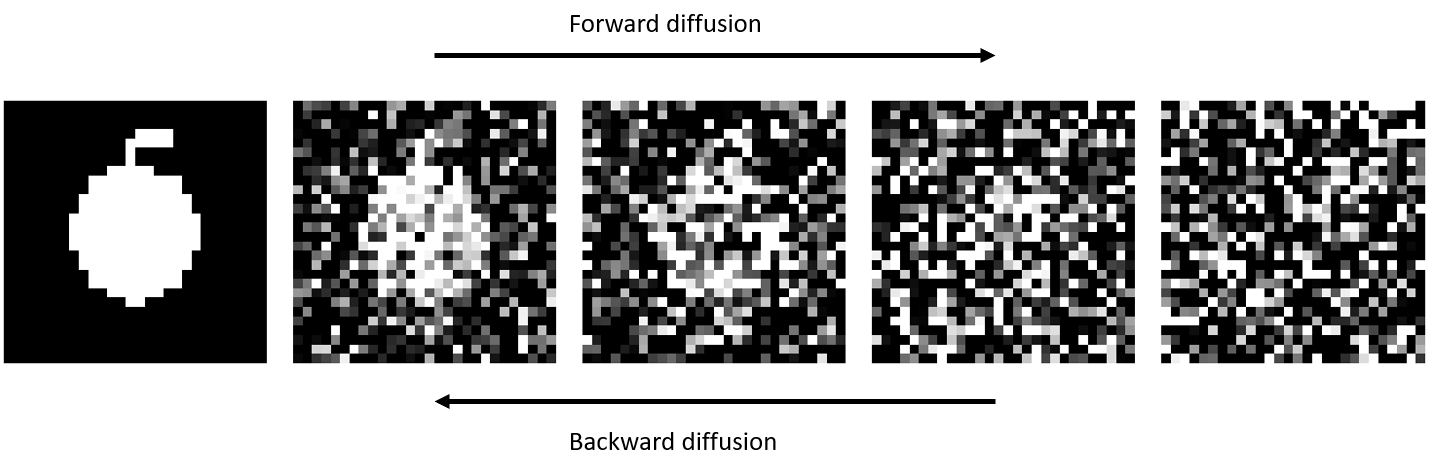
\includegraphics[width=\linewidth]{Figures/diffusion/forward_backward.png}
    \caption{First we created an image of an apple, and added noise step by step (forward diffusion). The reverse process is called backward diffusion.}
    \label{fig:appel_to_noise}
\end{figure}

Another example of diffusion, not from physics but from computer imaging, is the transformation of an image into noise. In every step, we add a square with random noise to our image. Every pixel is described with a number, and therefore we can add the random numbers of the noise to the (RGB) numbers that describe the image. In \cref{fig:apple_to_noise} we show it for a black and white image of an apple. When adding noise, the structure of the image slowly disappears.



The physical diffusion mechanism is called ``forward diffusion''.

\question{ Would it also be possible to reverse the physical process? For example, is it possible that all the scent in a room goes back to one point? Or for all milk in your coffee to gather in one corner of your cup? Also explain why.}


\subsection{Training the model}
The strength of AI diffusion models is that they learn how to do backward diffusion. They create a structured image out of random noise. Diffusion models can only do this by first understanding step-by-step how forward diffusion works. Therefore they are trained by observing forward diffusion in many examples. Then, starting with a random pixel grid, they can reverse this process and obtain an image.


 Training is done by trying something over and over again, and improving yourself until it works. Therefore the following steps are taken for many different images: all images in our training data. For example, we again take the image of the apple.
\begin{enumerate}
  \item First the model takes $N$ steps of forward diffusion, as is shown in \cref{fig:appel_to_noise}. This changes the apple into noise.
  \item It now focuses on one of the steps and tries to go in the other direction: to make a step in the reverse diffusion direction and make it look more like the apple. In other words, it tries to make some alterations to make the apple more visible, just like you did in the first activity.

\begin{figure}
    \centering
    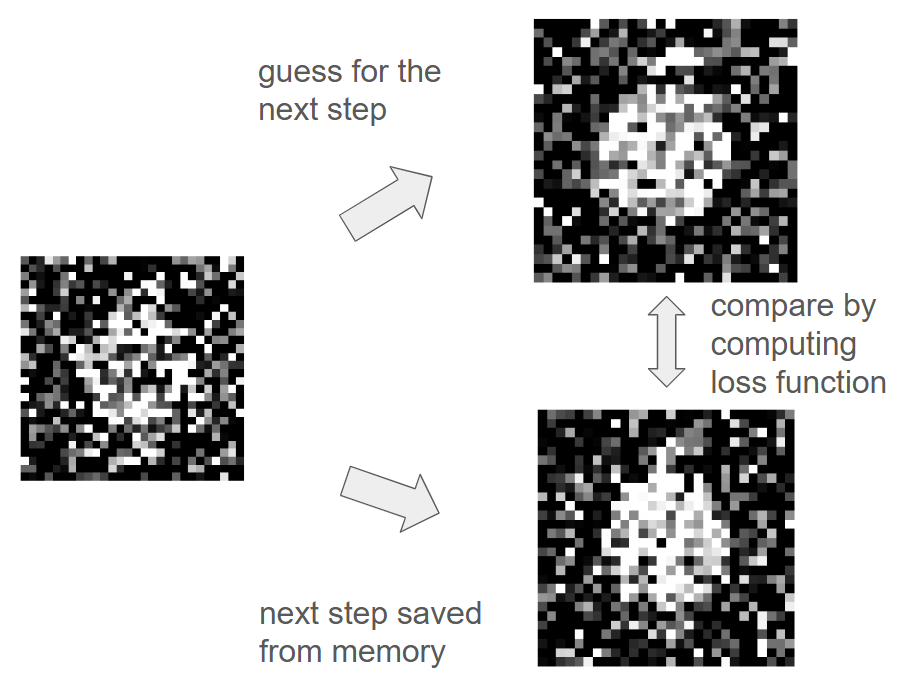
\includegraphics[width=0.7\linewidth]{Figures/diffusion/training.png}
    \caption{Training a diffusion model.}
    \label{fig:training}
\end{figure}
  
  \item The difference is, that the model has saved the precise image to end up with in its memory. Thus, it compares its prediction to the actual image from the previous step. The difference between these images is captured in a number, called the \emph{loss}. If the model is doing a perfect prediction, the loss will be $0$. If the loss is not $0$ yet, we change the model a little bit such that it will make a better prediction next time.
  \item We repeat this process for all the time steps, and for all training data, until the average loss is as low as we want it to be.
\end{enumerate}
This way, the model learns how to recover images from noise.

\subsection{Using the model for image generation}
When the model is trained long enough, it can be given a new challenge: we input a square with completely random noise. Now, we do not start with an image that we have hidden behind a lot of noise. Instead, the input is purely random.

We let the model work, and see what image it makes of the noise. Here, it will be a surprise what comes out, and it will heavily depend on the type of images that we used in our training data. If those were only images of butterflies, the model will also try to see a butterfly that is hidden in the noise.

In the image generation models we know, we can help the model with what type of image to find in noise. We input a text prompt. In the lesson on LLMs you learned how a computer translates this text to a vector.

So far we have ignored one thing. In our training and testing data, we saved a bit more information than just the image: we also labeled the image with a description of what is on it. Probably, you have helped putting these labels yourself when having to prove that you are not a robot, as in \cref{fig:captcha}.

\begin{figure}[h]
  \centering
  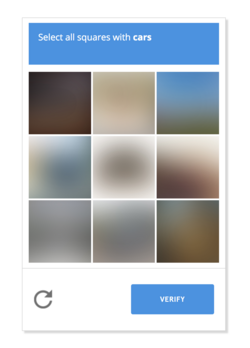
\includegraphics[width=0.4\linewidth]{Figures/diffusion/captcha.png}
  \caption{Often, we are helped to put labels on the training data for AI models.}
  \label{fig:captcha}
\end{figure}


The point is, that the model also learned which images correspond to which words (vectors). If you input a text prompt, it will search for an image in the noise that matches the words in your prompt.


\exercisetitle{Playing with Diffusion Models}
Go to \url{https://poloclub.github.io/diffusion-explainer/}. Try out what happens if you change:
\begin{itemize}
  \item The prompt
  \item Certain words in the prompt (by clicking on the underscore words)
  \item The guidance scale. This indicates how much the prompt is taken into account when generating the image.
  \item The seed. There are three different possible random noise starting images in this program.
\end{itemize}

Answer the following questions:

\question[4\baselineskip]{From which timestep do you start to see the image?}
\question[4\baselineskip]{When you compare two different versions of the same prompt, at what point do they start to vary?}
\question[4\baselineskip]{Why do the three different seeds lead to different images?}
\question[4\baselineskip]{Which setting of the guidance scale do you think works best? Why?}

\exercisetitle{Strengths and limitations of diffusion models}

Discuss the following questions in a small group. Be prepared to share your answers in class. 
\begin{itemize}
  \item Why do AI image generation models sometimes hallucinate?
  \item What aspects of image generation do you expect diffusion models to be good at?
  \item What could the diffusion mechanism be used for, apart from image generation?
\end{itemize}

\end{document}